\documentclass[12pt]{artikel3}                  % I need a font of 12 for the proposal.
\linespread{1.2}                                % Not sure why we need this here.
\usepackage{fullpage, setspace, graphicx}       % What does the full page library do?
\usepackage{mathtools, amsfonts}                % Mathtools are understandable, and so are the amsfonts that are being used.
\usepackage[margin=1in]{geometry}
\usepackage{newcent}                            % Why do I need the newcent package or what it does?
\usepackage{url}                                % If I am including URL in any place, I will need this package.
\usepackage{cite}                               % Need this for citing of the various formats.
\usepackage{hyperref}
\usepackage{algorithm}
\usepackage{algpseudocode}

\begin{document}
\begin{titlepage}
\begin{center}

\textsc{\LARGE }\\[0.2cm]
\textsc{\LARGE }\\[0.2cm]
\textsc{\LARGE }\\[1.2cm]

\textsc{\Large Master's Project Proposal}\\[1cm]

\large{Soham Sadhu}\\
\large{Department of Computer Science}\\
\large{Rochester Institute of Technology}\\
\large{Rochester, NY 14623}\\
\large{sxs9174@rit.edu}\\[0.5cm]

{\large \today}\\[1cm]

\begin{tabular}{l l r}
    Chair: & Prof. Stanis{\l}aw Radziszowski & spr@cs.rit.edu\\[1.5cm] \hline
    \multicolumn{3}{c}{signature \hspace{6cm} date}\\[1cm]
    Reader: & Prof. Alan Kaminsky & ark@cs.rit.edu\\[1.5cm] \hline
    \multicolumn{3}{c}{signature \hspace{6cm} date}\\[1cm]
    Observer: & Prof. Edith Hemaspaandra & eh@cs.rit.edu\\[1.5cm] \hline
    \multicolumn{3}{c}{signature \hspace{6cm} date}\\[1cm]
\end{tabular}


\vfill

\end{center}
\end{titlepage}

\begin{center}
\parbox{350pt}{
  \begin{center}\textsc{Abstract}\end{center}
  \vspace{0.5cm}
  Hash functions, have \href{"http://en.wikipedia.org/wiki/Cryptographic\_hash\_function\#Applications"}
  {applications in computer security}, in fields of authentication and integrity.
  Due to importance of hash function usage in everyday computing, standards for using hashing 
  algorithm and their bit size have been released by \href{"http://www.nist.gov/index.html"}
  {(NIST)} which are denoted by nomenclature Standard Hashing Algorithm (SHA).

  Due to advances in cryptanalysis of SHA-2, NIST announced a competition in November, 2007 
  to choose SHA-3. In October, 2012 the winner was selected to be \href{"http://keccak.noekeon.org/"}
  {Keccak} amongst 64 submissions. All the submissions were open to public scrutiny, and underwent
  intensive third party cryptanalysis, before the winner was selected. 
  \href{"http://csrc.nist.gov/groups/ST/hash/sha-3/sha-3\_selection\_announcement.pdf"}{Keccak was chosen}
   for its flexibility, efficient and elegant implementation, and large security margin.

  All algorithms submitted to competition have undergone public scrutiny. And other four finalist in 
  the competition were almost equivalent to Keccak, in attributes of security margin and implementation.
  In this project, I will be comparing Keccak with two other SHA-3 finalists, \href{"https://131002.net/blake/"}
  {BLAKE}, and \href{"http://www.groestl.info/"}{Gr$\o$stl} with respect to their resistance to 
  \href{"http://en.wikipedia.org/wiki/Simulated\_annealing"}{simulated annealing} and 
  \href{"http://en.wikipedia.org/wiki/Tabu\_search"}{tabu search}.
  
  Application of tabu search and simulated annealing to hash algorithms will be akin to generic attacks.
  That is these methods of breaking hash functions are design agnostic or do not depend on the workings
  of the hash function. Thus ensuring no bias in the experiment. At present, it is computationally infeasible
  to break the above mentioned hash functions. But the reduced versions of these can be subjected to attacks
  for near collisions. Thus I will be able to examine and conclude, if reduced instance Keccak has better 
  resistance to generic attacks than reduced instance of BLAKE and Gr$\o$stl.
}
\end{center}

\clearpage

\section{Problem Statement}

\subsection{Hash Functions}
A cryptographic hash function, is an algorithm capable of intaking arbitrarily long input string, and
output a fixed size string, often as called message digest. The message digest for two strings
even differing by a single bit should ideally be completely different, and no two input message should
have the same hash value. This property enables us to finger print a message. Following are the properties
of and ideal hash function\cite{00005}.
  
1. {\bf Preimage resistance}
\begin{center}
  \framebox
  {
    \parbox{350pt}
    {
      \centering \textsc{Preimage} \\
      {\bf Given:} A hash function $h : \mathcal{X} \to \mathcal{Y}$ and an element $y \in \mathcal{Y}$. \\
      {\bf Find:} $x \in \mathcal{X}$ such that $h(x) = y$. 
    }
  }
\end{center}
\vspace{4mm}
If the preimage problem for a hash function cannot be efficiently solved, then it is preimage resistant.
That is the hash function is one way, or rather it is difficult to find the input, given the output alone.

2. {\bf Second preimage resistance}
\begin{center}
  \framebox
  {
    \parbox{350pt}
    {
      \centering \textsc{Second preimage} \\
      {\bf Given:} A hash function $h : \mathcal{X} \to \mathcal{Y}$ and an element $x \in \mathcal{X}$. \\
      {\bf Find:} $x' \in \mathcal{X}$ such that $x' \neq x$ and $h(x) = h(x')$. 
    }
  }
\end{center}
\vspace{4mm}

A hash function for which a different input given another input, that compute to same hash cannot be found 
easily, is called as having second preimage resistance.

3. {\bf Collision resistance}
\begin{center}
  \framebox
  {
    \parbox{350pt}
    {
      \centering \textsc{Collision} \\
      {\bf Given:} A hash function $h : \mathcal{X} \to \mathcal{Y}$ 
      {\bf Find:} $x, x' \in \mathcal{X}$ such that $x' \neq x$ and $h(x') = h(x)$. 
    }
  }
\end{center}
\vspace{4mm}

Collision problem states that, can two different input strings be found, such that they hash to the same
 value given the same hash function. A hash function is collision resistant, if it is computationally
 infeasible to find two different values hashing to same value.

\subsection{Standards and NIST Competition}

Since hash functions can finger print any data, they find wide applications in computer security. And thus there
needs to be a standard for implemenation and application of hash function, which is provided by National Institute
of Standards and Technology(NIST). SHA-0 was initially proposed by National Security Agency(NSA) as a standardised
hashing algorithm in 1993. It was later standardised by NIST. In 1995 SHA-0 was replaced by SHA-1 designed by NSA
\cite{00006, 00007}. SHA-2 was designed by NSA, and released in 2001 by NIST. It is basically a family of hash 
functions consisting of SHA-224, SHA-256, SHA-384, SHA-512. The number suffix after the SHA acronym, indicates the 
bit length, of the output of that hash function. Although SHA-2 family of algorithms were influenced by SHA-1 
design, but the attacks on SHA-1 have not been successfully extended completely to SHA-2.

In response to advances made in cryptanalysis of SHA-2. NIST announced a public competition on November, 2007;
for a new cryptographic hash algorithm, that would be SHA-3. 51 candidates from 64 submissions for first round 
of competition were announced in December, 2008. In October, 2012 NIST announced the winner of the competition
to be Keccak, amongst the other four finalist, which were BLAKE, Gr$\o$stl, JH and Skein. Keccak was chosen for
its' large security margin, efficient hardware implementation, and flexibility.

\subsection{Motivation}

The arguments for choosing Keccak as SHA-3 are strong. However, other 4 finalists, have equally strong claim to
security margin; one of the attributes on which Keccak was chosen. All the finalists have gone public scrutiny,
and have shown resistance, to a number of attacks.

\vspace{3mm}
\begin{center}
  \framebox
  {
    \parbox{400pt}
    {
      \centering \textsc{Hypothesis} \\
      Reduced round Keccak, will have better resistance to near collisions found by tabu search and simulated
      annnealing, compared to reduced round BLAKE and Gr$\o$stl.
    }
  }
\end{center}
\vspace{3mm}

The aim of the project is to check if reduced version of Keccak holds security margin comparable, to reduced
versions of BLAKE and Gr$\o$stl. This will be done by subjecting the reduced versions of the 3 algorithms
to, a search in chaining value for two different messages. The search will be done in k-bit neighbourhood of
initial chaining value using tabu search and simulated annealing. This should lead to chaining values that can
give possible near collisions. These experiments would not prove that the said algorithms are vulnerable to 
attacks, but would rather provide a security margin on which they can be compared.
 
\clearpage

\section{Background}

\subsection{Gr$\o$stl}

Gr$\o$stl is collection of hash functions which produce digest size, ranging from 1 to 64 bytes. The variant of
Gr$\o$stl that returns a message digest of size n, is called Gr$\o$stl-n. Gr$\o$stl is an iterated hash function, 
with two compression functions named P and Q. The input is padded and then split into l-bit message blocks
$m_{1}$,$\ldots$, $m_{t}$, and each message block is processed sequentially. The initial l-bit chaining value 
$h_{0}$ = iv is defined, and the blocks $m_{i}$ are processed as $ h_{i}\gets f(h_{i-1}, m_{i})$ for i = 1,$\ldots$,
t. For variants up to 256 bits output, size of $l$ is 256 bits. And for digest sizes larger than 256 bits, $l$ 
is 1024 bits. After the last message block is processed, the last chaining value output is sent through a 
$\Omega$ function, to get the hash output H(M) \cite{00019}. 

$H(M) = \Omega(h_{t}),$

The f function shown above, is composed of two l-bit permutations called P and Q, which is defined as follows.

$f(h, m) = P(h \oplus m) \oplus Q(m) \oplus h.$

The $\Omega$ function consists of a $trunc_{n}(x)$ that outputs only the trailing n bits of input x. 
$\Omega(x) = trunc_{n}( P(x) \oplus x ).$

In order to fit the varying input length message to the block sizes of $ l $ padding is defined. First bit '1' is
appended, then $ w = -N - 65 mod l $ 0 bits are appended; where N is the length of the original message. Finally a
64 bit representation of $(N + w + 65) / l $.

There are two variations for P and Q permutations, one each for the digest size lower and higher than 256 bits. There
are four round transformations, that compose a round R. The permutation consists of a number of rounds R, and can be
represented as 

$ R = MixBytes \cdot ShiftBytes \cdot SubBytes \cdot AddRoundConstant $

The transformations SubBytes and MixBytes are same for all transformation while, ShiftBytes and AddRoundConstant differ
for each of the transformations. The transformations operate on matrix of bytes, with the permutation of lower size
digest having matrix of 8 rows and 8 columns, while that for larger variant is of 16 columns and 8 rows. The number of
rounds for digest sizes upto 256 bits are 10. For digest sizes higher than that, number of rounds are 14. The individual
components of each round for P and Q are described below.

{\bf AddRoundConstant:} transformation round XOR a round dependant constant to the state matrix say A. It is 
represented as $A \gets A \oplus C[i]$, where C[i] is the round constant in round i.

{\bf SubBytes:} substitutes each byte in state by value from S-box. Say $a_{i,j}$ a element in row i and column j of 
the state matrix, then the transformation done is $a_{i,j} \gets S( a_{i,j}),  0 \leq i < 8, 0 \leq j < v.$

{\bf ShiftBytes:} transformation cyclically shifts the bytes in a row to left by that number. Let list vector 
of a number denote the shift, with the index of the element indicating the row. The vector representation for
$P_{512}$ = [0, 1, 2, 3, 4, 5, 6, 7] and $Q_{512}$ = [1, 3, 5, 7, 0, 2, 4, 6]. Those for the larger permutation 
are $P_{1024}$ = [0, 1, 2, 3, 4, 5, 6, 11]and $Q_{1024}$ = [1, 3, 5, 11, 0, 2, 4, 6].

{\bf MixBytes:} transformation, multiplies each column of the state matrix A, by a constant 8 $\times$ 8 matrix B.
The transformation, can be shown as $ A \gets B \times A$. The matrix B, can be seen as a finite field over 
$\mathbb{F}_{256}$. This finite field is defined over $\mathbb{F}_{2}$ by the irreducible polynomial 
$x^{8} \oplus x^{4} \oplus x^{3} \oplus x \oplus 1$.

\subsection{BLAKE}

BLAKE\cite{00002} hash function is built on HAIFA (HAsh Iterative FrAmework) structure \cite{00020} which is an improved
version of Merkle-Damg$\dot{a}$rd function. BLAKE has 4 variations of the algorithm that can give only 4 different digest
lengths. The construction takes in 4 inputs, one message; two a salt, that makes function that parameter specific; and
three a counter, which is count of all the bits hashed till then; and lastly a chaining value which is input of the previous
operation or initial value in case of hash initiation. The compression function is composed of a 4 $\times$ 4 matrix of words.
Where one word is equal to 32 bits for BLAKE-256 variant, while 64 bit for variant BLAKE-512.

\begin{table}[h]
  \begin{center}
    \begin{tabular}{ c l } \hline
      Symbol                 & Meaning \\ \hline
      $\gets$                    & variable assignment \\
      $+$                    & addition modulo $2^{32}$ or (modulo $2^{64}$) \\
      $\gg k$                  & rotate k bits to least significant bits \\
      $\ll k$                  & rotate k bits to most significant bits \\
      $\langle l \rangle_{k}$ & encoding of integer $l$ over $k$ bits \\ \hline
    \end{tabular}
    \caption{Convention of symbols used in BLAKE algorithm}
  \end{center}
\end{table}

\subsubsection{ BLAKE-256 }

The compression function takes following as input
\begin{itemize}
  \item a chaining value of $h = h_{0},\dots, h_{7}$
  \item a message block $m = m_{0},\dots, m_{15}$
  \item a salt $s = s_{0},\dots, s_{3}$
  \item a counter $t = t_{0}, t_{1}$
\end{itemize}
These four inputs of 30 words or 120 bytes, are processed as $h' = compress(h, m, s, t)$ to provide a new
chain value of 8 words.

{\bf Compression function}

\begin{itemize}
\item {\bf Constants}
  \begin{table}[h]
    \begin{center}
      \begin{tabular}{ *{4}{c}}
        $IV_{0}$ = 6A09E667 & $IV_{1}$ = BB67AE85 & $IV_{2}$ = 3C6EF372 & $IV_{3}$ = A54FF53A \\
        $IV_{4}$ = 510E527F & $IV_{5}$ = 9B05688C & $IV_{6}$ = 1F83D9AB & $IV_{7}$ = 5BE0CD19 \\
      \end{tabular}
      \caption{Initial values which become the chaining value for the first message block}
    \end{center}
  \end{table}
  
  \begin{table}[h]
    \begin{center}
      \begin{tabular}{ *{4}{c}}
        $c_{0}$  = 243F6A88 & $c_{1}$  = 85A308D3 & $c_{2}$  = 13198A2E & $c_{3}$  = 03707344 \\
        $c_{4}$  = A4093822 & $c_{5}$  = 299F31D0 & $c_{6}$  = 082EFA98 & $c_{7}$  = EC4E6C89 \\
        $c_{8}$  = 452821E6 & $c_{9}$  = 38D01377 & $c_{10}$ = BE5466CF & $c_{11}$ = 34E90C6C \\
        $c_{12}$ = C0AC29B7 & $c_{13}$ = C97C50DD & $c_{14}$ = B5470917 & $c_{15}$ = 3F84D5B5 \\
      \end{tabular}
      \caption{16 constants used for BLAKE-256}
    \end{center}
  \end{table}

  \begin{table}
    \begin{center}
      \begin{tabular}{ c| *{16}{c}} \hline
        $\sigma_{0}$ & 0  & 1  & 2  & 3  & 4  & 5  & 6  & 7  & 8  & 9  & 10 & 11 & 12 & 13 & 14 & 15 \\
        $\sigma_{1}$ & 14 & 10 & 4  & 8  & 9  & 15 & 13 & 6  & 1  & 12 & 0  & 2  & 11 & 7  & 5  & 3  \\
        $\sigma_{2}$ & 11 & 8  & 12 & 0  & 5  & 2  & 15 & 13 & 10 & 14 & 3  & 6  & 7  & 1  & 9  & 4  \\
        $\sigma_{3}$ & 7  & 9  & 3  & 1  & 13 & 12 & 11 & 14 & 2  & 6  & 5  & 10 & 4  & 0  & 15 & 8  \\
        $\sigma_{4}$ & 9  & 0  & 5  & 7  & 2  & 4  & 10 & 15 & 14 & 1  & 11 & 12 & 6  & 8  & 3  & 13 \\
        $\sigma_{5}$ & 2  & 12 & 6  & 10 & 0  & 11 & 8  & 3  & 4  & 13 & 7  & 5  & 15 & 14 & 1  & 9  \\
        $\sigma_{6}$ & 12 & 5  & 1  & 15 & 14 & 13 & 4  & 10 & 0  & 7  & 6  & 3  & 9  & 2  & 8  & 11 \\
        $\sigma_{7}$ & 13 & 11 & 7  & 14 & 12 & 1  & 3  & 9  & 5  & 0  & 15 & 4  & 8  & 6  & 2  & 10 \\
        $\sigma_{8}$ & 6  & 15 & 14 & 9  & 11 & 3  & 0  & 8  & 12 & 2  & 13 & 7  & 1  & 4  & 10 & 5  \\
        $\sigma_{9}$ & 10 & 2  & 8  & 4  & 7  & 6  & 1  & 5  & 15 & 11 & 9  & 14 & 3  & 12 & 13 & 0  \\ \hline
      \end{tabular}
      \caption{Round permutations to be used}
    \end{center}
  \end{table}

\item {\bf Initialization: } The constants mentioned are used with the salts, and counter along with initial
value used as chaining input, to create a initial matrix of 4 $\times$ 4, 16 word state.

$\begin{pmatrix} v_{0} & v_{1} & v_{2} & v_{3} \\ v_{4} & v_{5} & v_{6} & v_{7} \\
                 v_{8} & v_{9} & v_{10} & v_{11} \\ v_{12} & v_{13} & v_{14} & v_{15}\end{pmatrix} 
\gets
\begin{pmatrix} h_{0} & h_{1} & h_{2} & h_{3} \\ h_{4} & h_{5} & h_{6} & h_{7} \\
   s_{0} \oplus c_{0} & s_{1} \oplus c_{1} & s_{2} \oplus c_{2} & s_{3} \oplus c_{3} \\ 
   t_{0} \oplus c_{4} & t_{0} \oplus c_{5} & t_{1} \oplus c_{6} & t_{1} \oplus c_{7} \end{pmatrix}$

\item {\bf Round function:} After initialisation, the state is subjected to column and diagonal operations, 14
times. A round operation G acts as per following

\begin{table}
  \begin{center}
    \begin{tabular}{ *{4}{c}}
    $ G_{0}(v_{0}, v_{8}, v_{12})$ & $G_{1}(v_{1}, v_{5}, v_{9}, v_{13})$ & $G_{2}(v_{2}, v_{6}, v_{10}, v_{14})$ & $G_{3}(v_{3}, v_{7}, v_{11}, v_{15}) $\\
$G_{4}(v_{0}, v_{5}, v_{10}, v_{15})$ & $G_{5}(v_{1}, v_{6}, v_{11}, v_{12})$ & $G_{6}(v_{2}, v_{7}, v_{8}, v_{13})$ & $G_{7}(v_{3}, v_{4}, v_{9}, v_{14})$
    \end{tabular}
  \end{center}
\end{table}

where the round function $G_{i}(a, b, c, d)$ sets

$
a \gets a + b + (m_{\sigma_{r}(21)} \oplus c_{\sigma_{r}(2i + 1)}) \\
d \gets (d \oplus a) \gg 16 \\
c \gets c + d \\
b \gets (b \oplus c) \gg 12 \\
a \gets a + b + (m_{\sigma_{r}(2i + 1)} \oplus c_{\sigma_{r}(2i)}) \\
d \gets (d \oplus a) \gg 8 \\
c \gets c + d \\
b \gets (b \oplus c) \gg 7
$

The implementation of the G function is shown below.
\begin{figure}[h]
  \begin{center}
    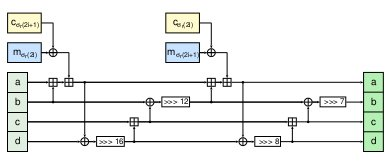
\includegraphics[width=4in]{blakeGfunction.jpg}
  \end{center}
  \caption{The $G_{i}$ function in BLAKE}
  \label{fig:lab}
\end{figure}

\item {\bf Finalization:} The chaining values for the next stage are obtained by XOR of the words from the state 
matrix, the salt and the initial value.

$
h'_{0} \gets h_{0} \oplus s_{0} \oplus v_{0} \oplus v_{8} \\
h'_{1} \gets h_{1} \oplus s_{1} \oplus v_{1} \oplus v_{9} \\
h'_{2} \gets h_{2} \oplus s_{2} \oplus v_{2} \oplus v_{10} \\
h'_{3} \gets h_{3} \oplus s_{3} \oplus v_{3} \oplus v_{11} \\
h'_{4} \gets h_{4} \oplus s_{0} \oplus v_{4} \oplus v_{12} \\
h'_{5} \gets h_{5} \oplus s_{1} \oplus v_{5} \oplus v_{13} \\
h'_{6} \gets h_{6} \oplus s_{2} \oplus v_{6} \oplus v_{14} \\
h'_{7} \gets h_{7} \oplus s_{3} \oplus v_{7} \oplus v_{15} \\
$
\end{itemize}

{\bf Hashing the message}

A given input message is padded with a bit '1' followed followed by at most 511 bits of zeros, so that the message 
size is equal to 447 modulo 512. This padding is followed by a bit '1' and a 64-bit unsigned big-endian representation
of block length $l$. The padding to a message, can be represented as $m \gets m \parallel 1000 \dots 0001\langle l \rangle_{64}$

\begin{algorithm}
\caption{BLAKE Compression procedure}
\begin{algorithmic}[1]
\State $ h^{0} \gets IV $
\For {$i = 0,\dots, N - 1$}
  \State $h^{i+1} \gets compress(h^{i}, m^{i}, s, l^{i})$
\EndFor
\State\Return{$h^{N}$}
\end{algorithmic}
\end{algorithm}

As shown in algorithm 1, the BLAKE compression function ingests the padded message block by block, in a loop 
starting from the initial value, and then sends the last chained value obtained from the finalization to the 
$\Omega$ truncation function, to obtain the hash value.

\subsection{Keccak}


\section{Related Work}

\section{Methodology}

\section{Evaluation and expected outcomes}

\bibliographystyle{plain}
\bibliography{CapstoneBib}

\end{document}
